\documentclass{bioinfo}
\copyrightyear{2005}
\pubyear{2005}

\begin{document}
\firstpage{1}

\title[The Functional Therapeutic Chemical Classification System]{The Functional Therapeutic Chemical Classification System}
\author[Croset \textit{et~al}]{Samuel Croset\,$^{1, \footnote{to whom correspondence should be addressed}}$, John Overington\,$^{1}$ and Dietrich Rebholz-Schuhmann\,$^{1}$
}
\address{$^{1}$European Molecular Biology Laboratory
European Bioinformatics Institute (EMBL-EBI), Wellcome Trust Genome Campus, Hinxton, Cambridge CB10 1SD,
United Kingdom\\}

\history{Received on XXXXX; revised on XXXXX; accepted on XXXXX}

\editor{Associate Editor: XXXXXXX}

\maketitle

\begin{abstract}


\section{Motivation:}
Drug repurposing is the discovery of new indications for compounds already approved and used in a clinical setting. 
Recently, some computational approaches have been developed to unveil new opportunities in a systematic fashion, by taking 
into consideration gene expression signatures or chemical features for instance. 
We present here a novel method based on knowledge integration using semantic technologies. 
In order to computationally generate repurposing hypotheses, we used the Web Ontology Language (OWL) to 
mathematically define the meaning of over 20'000 terms formally describing various modes and mechanisms of action.

\section{Results:}
Based on an integration of public data, we have automatically assigned over a thousand of approved drugs into 
these mode of action categories. The resulting new resource is called the Functional Therapeutic Chemical Classification System (FTC) 
and was further evaluated against the content of the traditional Anatomical Therapeutic Chemical Classification System (ATC). 
We illustrate how the new classification can be used to generate drug repurposing hypotheses, using Alzheimer’s disease as a use-case.

\section{Availability:} A web application built on the top of the resource is freely available at {{https://www.ebi.ac.uk/chembl/ftc}}. The 
source code of the project is available at {{https://github.com/loopasam/ftc}}.

\section{Supplementary Information:}
Supplementary data are available at Bioinformatics online.

\section{Contact:} \href{croset@ebi.ac.uk}{croset@ebi.ac.uk}
\end{abstract}

\section{Motivation}

Drug repurposing is the use of known active compounds for new therapeutic indications \citep{Sanseau01072011}. 
When administered in a living organism, a compound can indeed play various roles and affect different biological processes. 
Accurately identifying these different functions helps to predict the potential side-effects a drug could have and can also lead to 
interesting repurposing opportunities \citep{Medina-Franco2013}. For instance, sildenafil was initially developed 
against angina and has been repurposed towards erectile dysfunction during the clinical trials \citep{Ashburn2004}. Approved compounds are 
attractive because they have been extensively studied and have by definition already successfully passed clinical trials, where 
most drugs fail because of safety or efficacy issues.
There is an increasing number of approaches to predict repurposing opportunities using computational methods \citep{Sanseau01072011}. Most 
methods operate on the profiles of physicochemical descriptors derived from molecular structures \citep{Haupt2011}. Other methods characterise 
the drugs on more abstract levels, such as the gene expression signature \citep{Iorio2010} or 
via the reported side-effects \citep{Campillos2008}. 
These approaches 
have in common to look for similarities within existing drugs and forward similar compounds as repurposing hypotheses.
A feature of particular interest to describe drugs is the mode of action (MoA). According to Wikipedia, 
the MoA describes a functional or anatomical change, 
at the cellular level, resulting from the exposure of a living organism to a substance. For instance 
terms such as transcriptional regulation agent or anticoagulant define MoAs and characterise the roles of a certain type of drugs. The 
MoA abstracts over the relations between molecular functions, protein targets and drug activities; it is the central concept linking a 
chemical structure to a set of biological effects. Intuitively, the indication of a drug logically depends on its MoA.
Despite its widespread use in drug discovery, the MoA has not been used yet as a descriptor for repurposing analyses. One reason for this 
might be the challenge of formally defining MoAs. Indeed, MoAs are terms or categories, it is not possible to represent 
them straightforwardly with values and numbers like one can do for a 3D molecular structure or for a gene expression profile. 
Nonetheless, the meaning of a concept can be formalised with controlled vocabularies and ontologies \citep{Gruber1995}; 
originating from description logics, such frameworks help to define the mathematical meaning of symbols and strings of characters. 
In an ontology or knowledge base, concepts are organised and linked following the logical type of relation they have between them. 
In the Gene Ontology (GO) for example \citep{Ashburner2000}, biological processes and molecular functions are manually curated in this resource 
and the meaning of terms is specified by the relations linking two GO terms.
MoA definitions are present in other classifications such as the Medical Subject Headings \citep{Nelson2004} or the Chemical Entities of 
Biological Interest \citep{Hastings2012} for example. The Anatomical Therapeutic 
Chemical Classification System (ATC) \citep{world2000anatomical} also describes to some 
extent the action of drugs at the anatomical level. All these resources are valuable for the community as a source of carefully 
manually curated information. Moreover, the categories described in these classification systems are sometimes used to annotate 
drugs: For instance the compound sildenafil has been manually annotated as vasodilator agent (CHEBI:35620 or MeSH:D27.505.954.411.918).
The classifications mentioned previously are not specially designed for drug repurposing; they purposefully report only the 
well-known and major MoAs of chemical compounds. The pharmacological spectrum of each drug is not necessarily well covered, yet 
it would be the best way to predict new indications. In our context, an ideal knowledge base would feature the known MoAs of a 
drug as well as some predicted ones to be tested in experiments. The MoA categories should derive and scale over primary molecular 
evidences exposed in biomedical databases in an automated way.
To address the lack of systematic MoA annotations, we have implemented the Functional Therapeutic Chemical 
Classification System (FTC), presented here in this manuscript. The FTC is automatically built by leveraging the content 
of various biomedical databases using description logics and automated reasoning. Over 20'000 new MoA categories are defined 
in the resource and further populated with approved drugs using the Web Ontology Language (OWL) in combination with a reasoner. 
Most of the drugs are present in multiple FTC categories, reflecting the various roles a compound can play inside a biological system. 
The resource was evaluated against the ATC, traditional classification scheme introduced before. We present as well some preliminary 
analyses over the data, by looking at the relation between the MoA and the indication of a compound using semantic similarity. 
Finally, we illustrate also how the FTC can be used as a pharmacological toolbox to analyse drug repurposing for Alzheimer’s disease.

\section{Results}

The knowledge base behind the FTC is built by integrating information coming from various sources. 
The GO terms serve as template to create the FTC categories describing the MoAs; DrugBank provides the 
known links between drugs and their protein targets. Uniprot maps targets to their respective GO annotations. 
Drugs are further assigned into mode of action categories based of the OWL constructs and axioms defined in the 
FTC (see Availability and Implementation). A reasoner, a program capable of understanding such axioms, performed this task. 
The process to build the FTC is summarised in Figure~\ref{fig:01}.

\begin{figure*}[!tpb]%figure1
\centerline{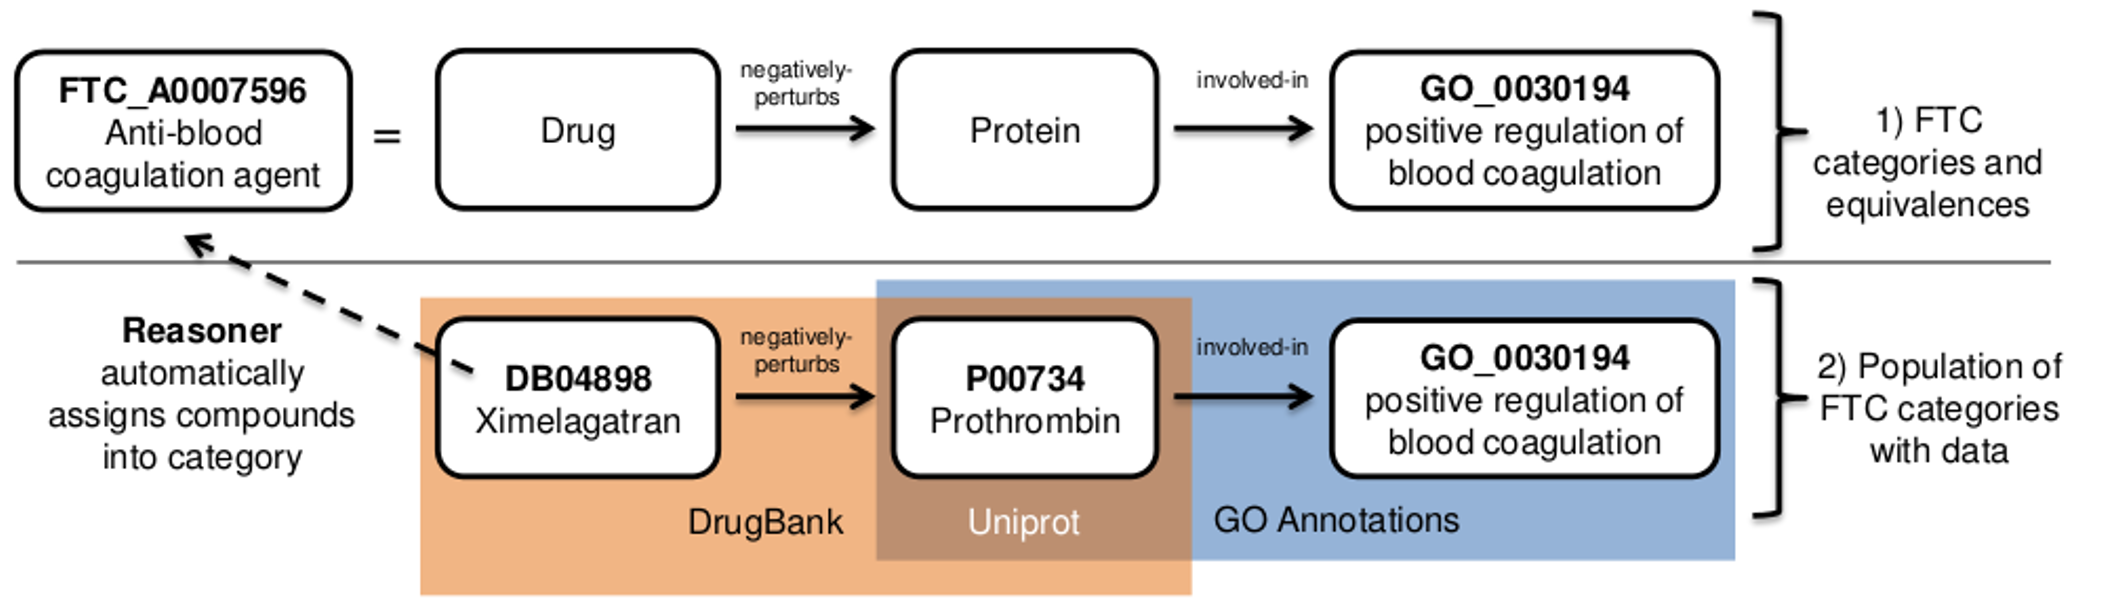
\includegraphics{fig1.png}}
\caption{Parent categories to the FTC class Pro-fibrinolysis agent (FTC\_P0042730). The classification is a direct 
acyclic graph where categories are describing increasingly specific concepts. Arrows entails subclass relationships 
between the terms (is a relation).}\label{fig:01}
\end{figure*}

It takes around 5 seconds on a modern 
laptop (4 cores processor with 4 Gb of memory) to classify the knowledge base using the ELK reasoner (cite). 
Other OWL reasoners have been tried (e.g, Hermit (cite), Pellet (cite), etc...) but none of them were suitable for this purpose; 
the classification time was always superior to a few minutes (data not shown). The FTC has a taxonomic structure as illustrated 
on Figure~\ref{fig:02}, which arises when the reasoner classifies the knowledge base. Categories can have multiple parents and multiple children. 
The reader can browse and access the content of the FTC online at {{https://www.ebi.ac.uk/chembl/ftc}}.

\begin{figure}[!tpb]%figure2
\centerline{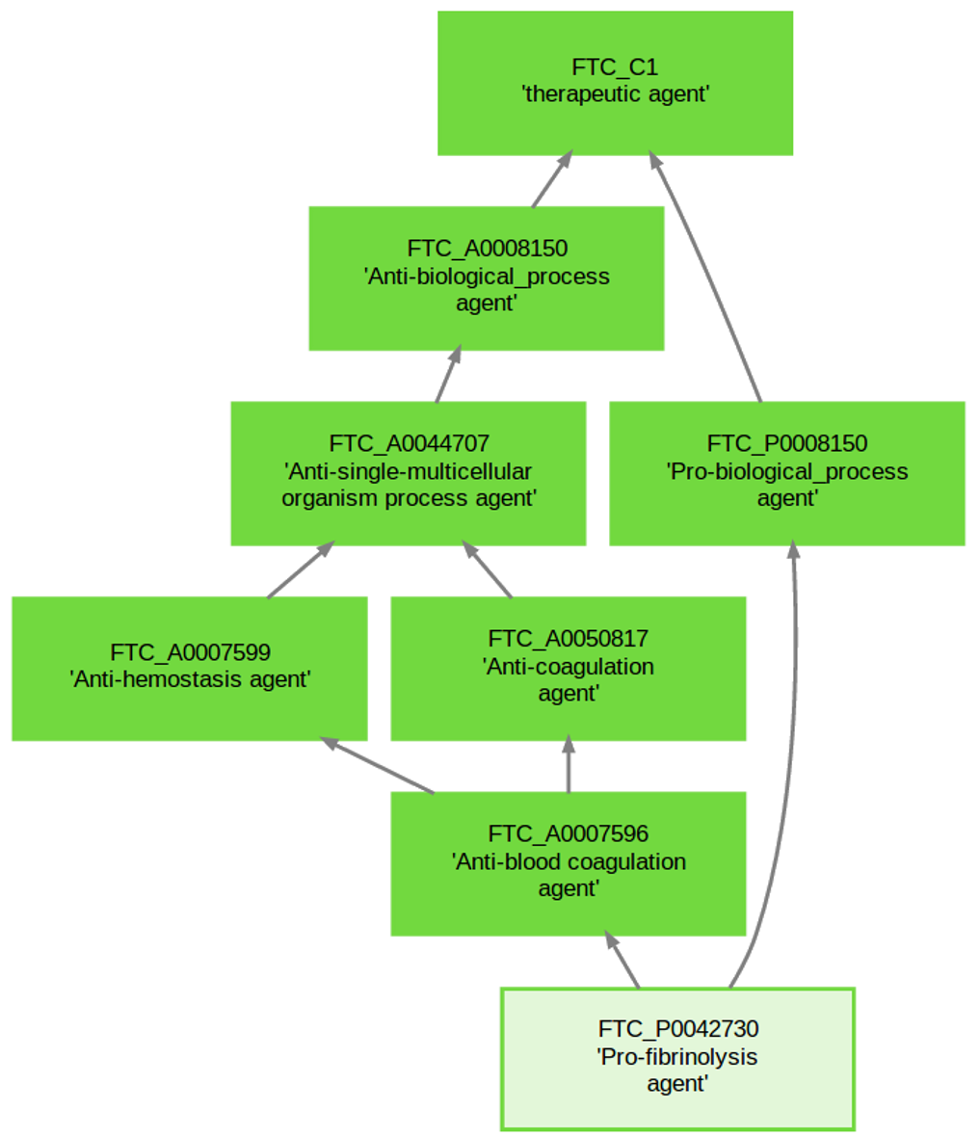
\includegraphics{fig2.png}}
\caption{Parent categories to the FTC class Pro-fibrinolysis agent (FTC\_P0042730). The classification is a direct 
acyclic graph where categories are describing increasingly specific concepts. Arrows entails subclass relationships 
between the terms (is a relation).}\label{fig:02}
\end{figure}

In total there are 1280 approved DrugBank compounds (chemical and biotherapeutics) perturbing 1264 human protein targets. 
The FTC introduces 23'353 new categories describing the mode and mechanism of action of therapeutic compounds. 4289 of these 
categories are related to biological processes and 19'064 to the molecular functions. A summary of the metrics behind the latest 
build is available online at {{https://www.ebi.ac.uk/chembl/ftc/evaluation/}}. Out of all FTC classes, 1432 
categories (\textgreater 6\%) directly contain at least one approved drug. This number increases up to 2532 (\textgreater 11\%) 
when direct and 
indirect drugs are considered. FTC categories not containing drugs (e.g, FTC\_A0001771 - Anti-immunological synapse 
formation agent) represent modes and mechanisms of action for which no approved compounds exist yet or that have not been identified 
as such in the FTC.

\subsection{Evaluation}
The content of the FTC has been evaluated against the information present in the ATC. The motivation behind 
this step is to have an estimation of how the automatically-built classification (FTC) compares to a manually curated 
one (ATC). In the context of this work, we have considered the ATC as a gold standard against which the FTC 
has been assessed. In practice, these two resources have different goals; therefore the evaluation should be 
interpreted accordingly. The full methodology behind the evaluation is described in the section “Evaluation methodology”. 
Briefly, 68 classes present in the FTC have an equivalent meaning to a combination of classes present in the ATC. 
This semantic equivalence was manually asserted and called evaluation point (see “Evaluation points” from Availability and Implementation). 
The set of drugs present in both classes for each evaluation points were then compared and some metrics are derived 
from this comparison. For example, the FTC category Anti-hydrogen:potassium-exchanging ATPase activity agent (FTC\_A0008900) has 
been manually asserted as equivalent to the ATC category Proton pump inhibitors (A02BC). A summary of this 
evaluation point is furthermore available online at {{https://www.ebi.ac.uk/chembl/ftc/evaluation/FTC\_A0008900}}.
Out of the 1280 DrugBank compounds present in the FTC, 1134 are also present in the ATC, therefore only those were 
considered. The evaluation points cover a total of 471 DrugBank compounds. Out of these, 277 compounds are true positives, 
meaning that given an evaluation point, they are present in both FTC and ATC categories. The proton pump inhibitor 
evaluation point is such an example where all the drugs (omeprazole, esomeprazole, pantoprazole, lansoprazole, rabeprazole) are 
present both in the FTC category and in the corresponding ATC class. The total number of compounds presents in an ATC class but 
not in the corresponding FTC category (false negatives) is 36. Finally, 279 compounds are present in a FTC class but not in the 
corresponding ATC class; such agents are the false positives. From these values, it is possible to derive a 
recall of 88\%; this percentage indicates that the automatic build of the FTC covers a good portion of the content 
already present in the ATC. The precision of 50\% shows that the FTC contains for a given MoA many more drugs than the 
equivalent ATC categories.

\subsection{Exploration}
The FTC was designed to assist drug repurposing analyses by explicitly representing the poly-pharmacology of 
approved drugs. In this section we exemplify how the resource can be used to perform different types of analysis.

\subsubsection{Polypharmacology spectrum}
With more information on a drug’s molecular targets and their physiological roles, the more opportunities 
exist to re-orient a drug into doing something new. The therapeutic agents described in the FTC can have several MoAs, 
representing the intrinsic polypharmacology of the approved compounds. Figure 2 illustrates the poly-pharmacology 
spectrum by showing the distribution of number of MoAs per compound. This number ranges from one to more 
than eighty for certain drugs, when indirect parents are considered. Not all the MoAs are biologically relevant, 
some FTC categories are particularly abstract (e.g, Anti-biological process agent) yet they represent discrete 
categories to which the drug belongs with an explicit and clear meaning. These discrete MoAs are a good starting 
point to understand what a compound can do when administered in a human system. The human readable definitions 
associated to each FTC category furthermore help the user to choose the adequate MoA for the desired outcome.

\begin{figure*}[!tpb]%figure3
\centerline{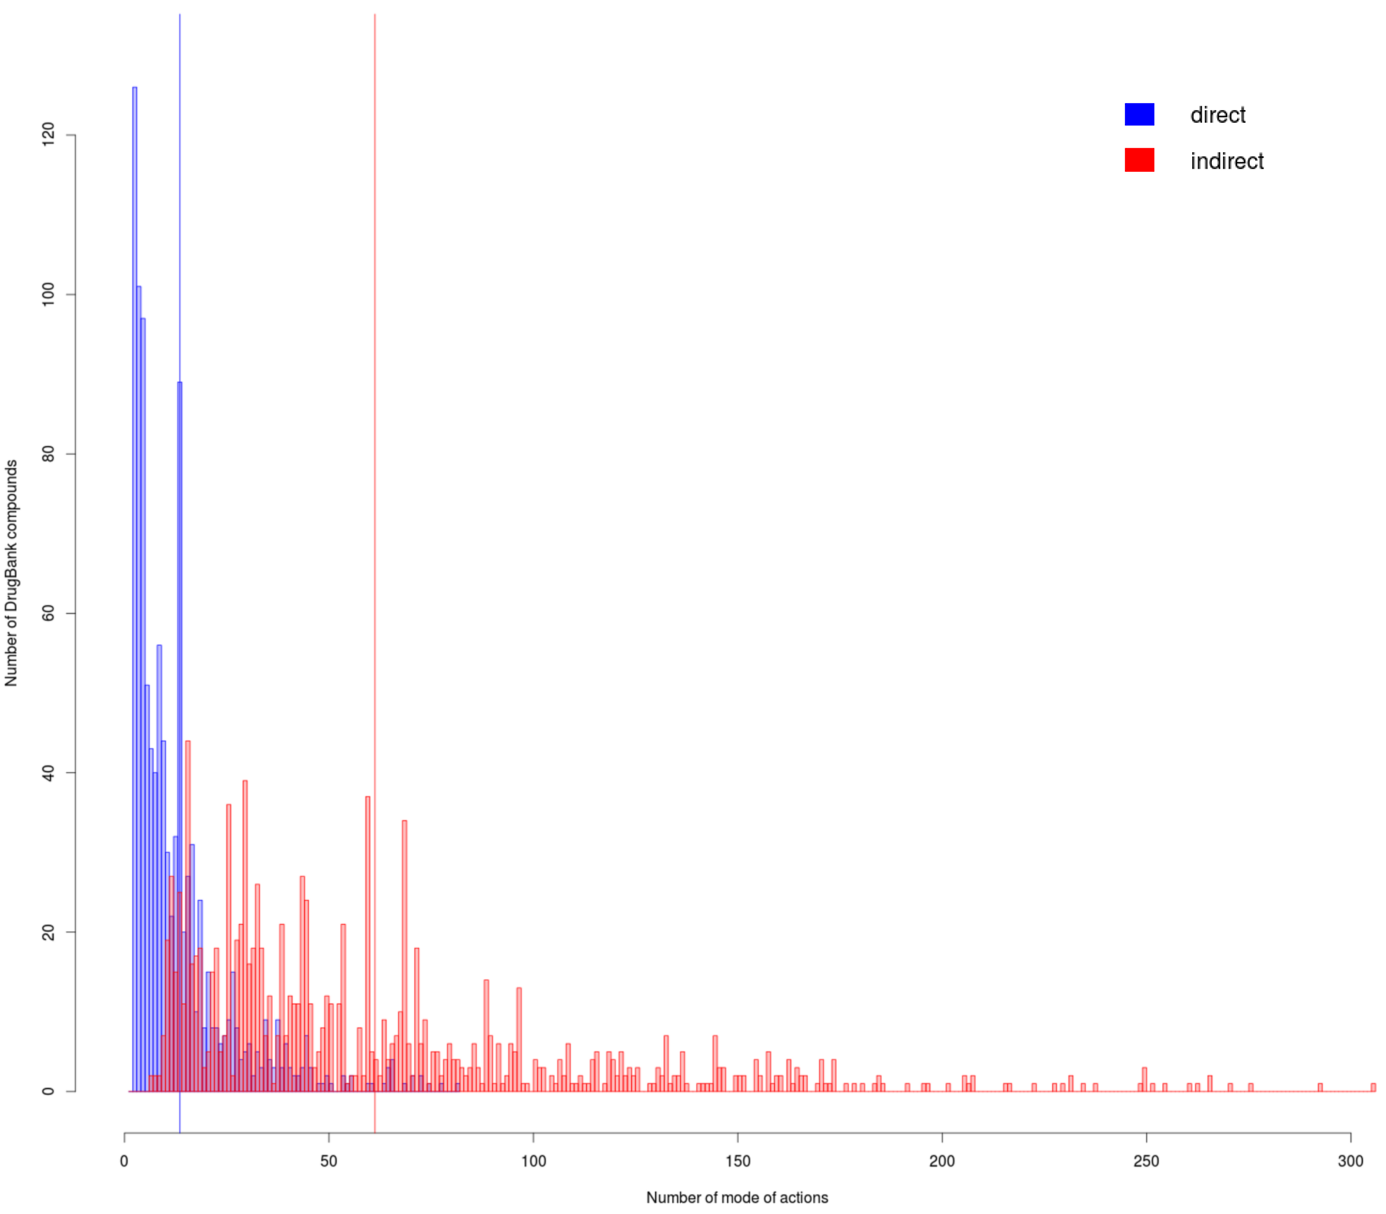
\includegraphics{fig3.png}}
\caption{Distribution of the direct and indirect number of MoAs per drug. 
Means are indicated with a solid line. When considering indirect categories, the distribution range is wider.}\label{fig:03}
\end{figure*}

\subsubsection{Drugs with similar mode of actions have similar indications}
The list of MoAs attributed to a drug can be exploited as a descriptor for the therapeutic agent. 
The tree structure of the FTC can be used to derive some similarity metrics over the MoAs. The underlying 
heuristic is to assume that the closer two entities are in a taxonomy or ontology, the more similar they are. 
We used a straightforward approach derived from the Jaccard index (see method for more details) in order to compare 
approved drugs based on the similarity of their MoAs. For instance, the similarity between two compounds present in 
the same FTC category is 1 (maximum). The similarity between an anti-blood coagulant and pro-blood coagulant is 0.29, 
reflecting the fact that such compounds are dissimilar in regards to the outcome of their biological effect. As the MoA is 
intuitively expected to be the central concept leading to the indication of the drug, we expected that on average, drugs with 
similar MoAs would be indicated towards similar therapeutic areas. The heat map presented in Figure 3 shows a pairwise 
comparison of all the drugs of the FTC based on their relative MoA similarity. The compounds are further grouped by 
therapeutic indications as defined by the ATC.

\begin{figure*}[!tpb]%figure4
\centerline{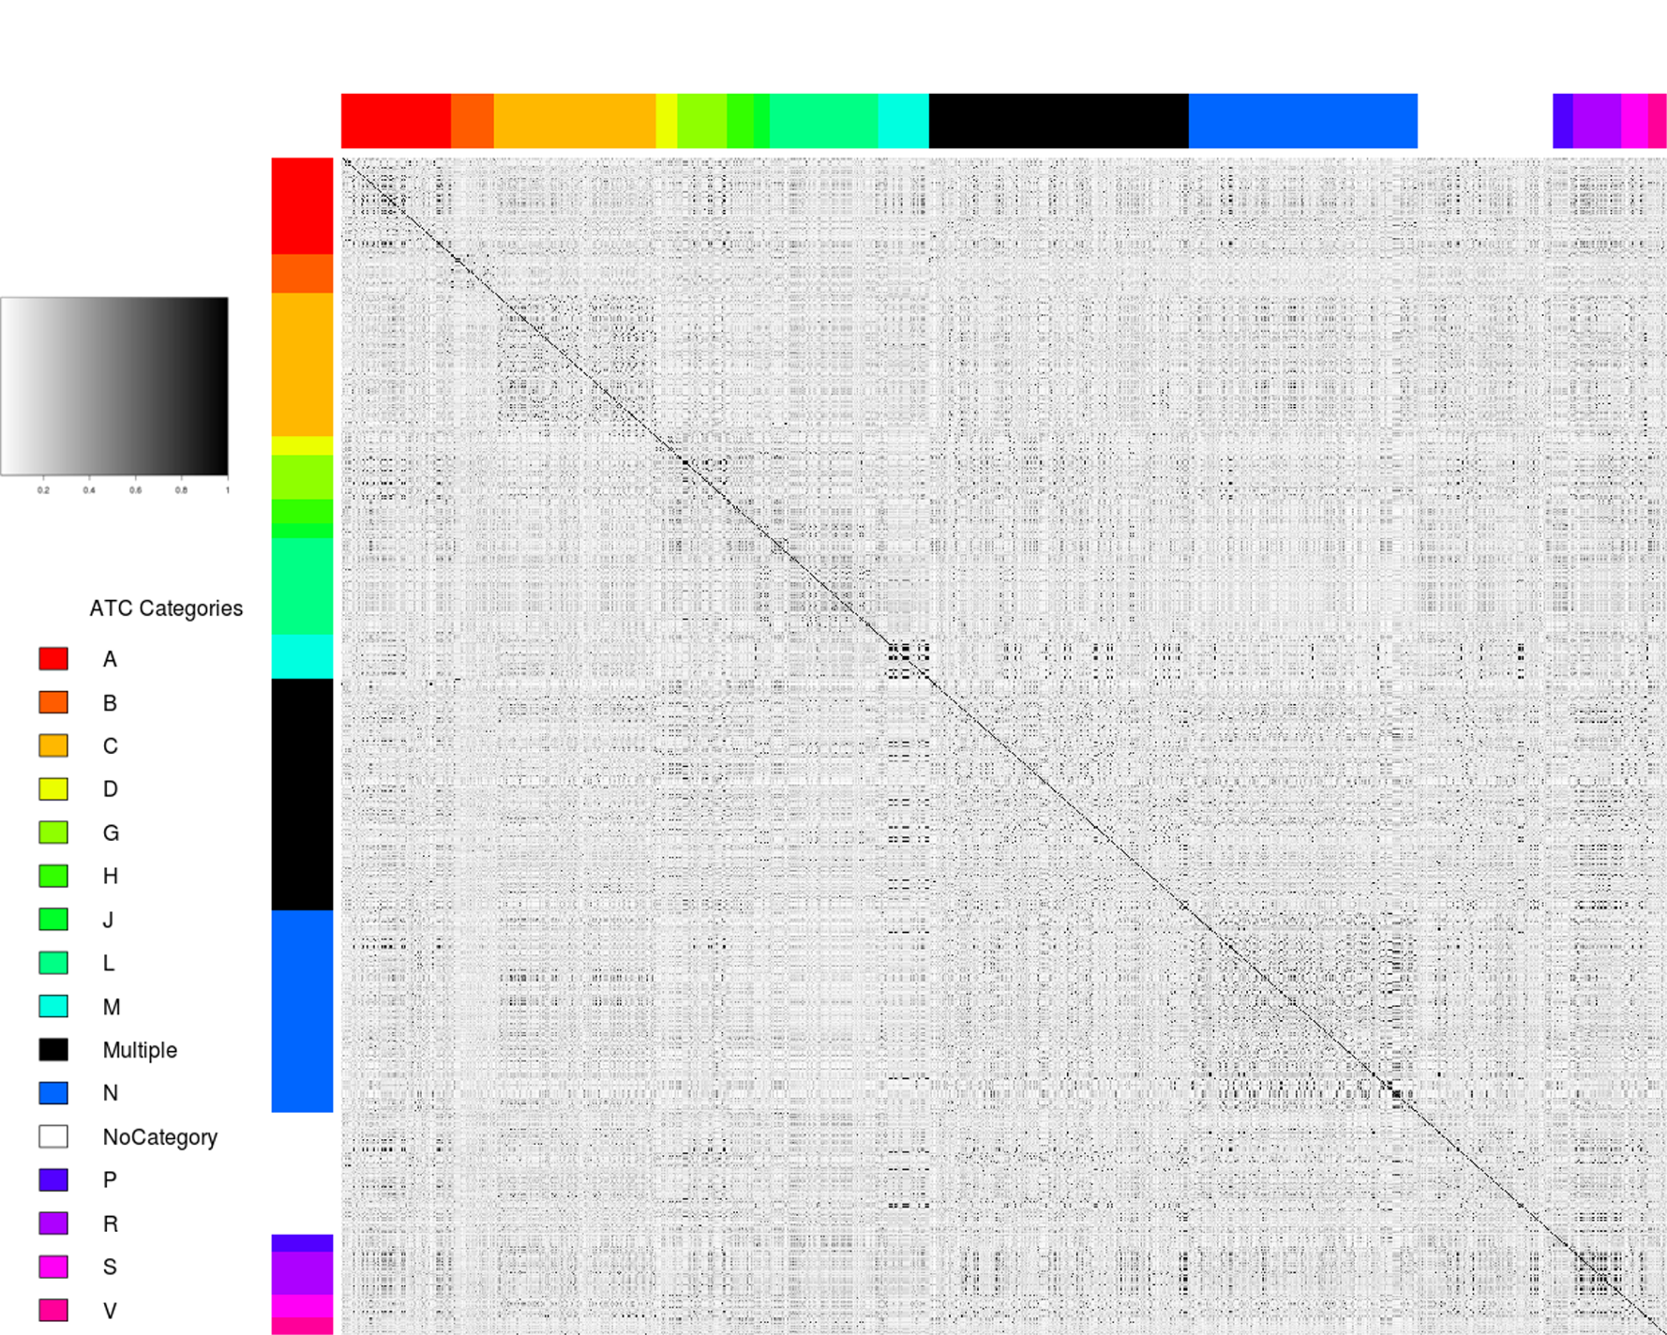
\includegraphics{fig4.png}}
\caption{Pairwise comparison of mode of action similarities. Only the first level of 
the ATC is considered. The reader can refer to Supplementary Figure 1A for a two ATC level granularity. 
The similarity descriptor ranges from 0 (not similar - white) to 1 (identical - black). Drugs are grouped according 
to their first ATC level (colours on the side). For instance, the compound reteplase (DB00015) has the ATC code B01AD07, 
which appears as “B” (dark orange) on the plot. The average similarity of drugs present in the same therapeutic category 
is significantly higher on average when separately compared to all other indications.}\label{fig:04}
\end{figure*}

The heat map displayed in Figure 3 reveals some square patches around the central diagonal. 
The overall similarity appears higher when compounds from the same ATC group are considered. 
A significance analysis (cf details covered in sections “Semantic similarity” 
and “Mode of action similarity against indication” from Availability and Implementation) 
revealed that the average MoA similarity of compounds belonging to the same ATC category is 
significantly higher than when compounds belonging to different categories are compared. Indeed, for 
each category, the p-value was inferior to 0.05 based on 20'000 random permutations over the similarity values. 
This result supports the idea that drugs with similar MoAs have similar indications. Note that the mean of the 
similarity values was considered for the statistical analysis; some outliers are also present in the map, which 
can be interpreted as repurposing hypotheses. These outliers have indeed similar MoAs, yet they belong to totally 
different therapeutic areas and are used for different purposes according to the ATC. We are currently further analysing 
such cases in a systematic fashion. Supplementary Figure S1A present similar association behavior when two levels of the ATC are 
considered (no statistical significance performed). Supplementary Figure S1B re-uses the same data as Figure 1 (one ATC level) 
but with a clustering function apply to it (hierarchical clustering - manhattan distance) in order to reveal 
functional clusters of drugs. Finally, Figure S1C shows the distribution when compounds are sorted based on 
their identifiers; no patterns are identifiable in this case. Taken together, these results emphasize that the MoAs as 
defined in the FTC are indeed on average associated with the therapeutic indication of a drug.
 
\subsection{Drug repurposing hypotheses for Alzheimer’s disease}
In this section we provide examples how actual drug repurposing hypotheses can be derived from the FTC. 
The approach presented here makes use of the FTC categories as analogs to compartments of a toolbox helping to 
find drugs to treat Alzheimer’s disease. Five FTC categories containing drugs are directly related to the biological 
processes of the neurodegenerative condition: Anti-amyloid precursor protein biosynthetic process agent (FTC\_A0042983), 
Anti-tau protein kinase activity agent (FTC\_A0050321), Anti-tau protein binding agent (FTC\_A0048156), Anti-beta amyloid 
binding agent (FTC\_A0001540) and Pro-beta amyloid binding agent (FTC\_P0001540). We have then considered the drugs present 
inside each of these classes as potential candidates. Figure 4 shows these drugs, which have been further manually grouped 
based on the overall similarity of their actions (letters on Figure 4).

\begin{figure}[!tpb]%figure5
\centerline{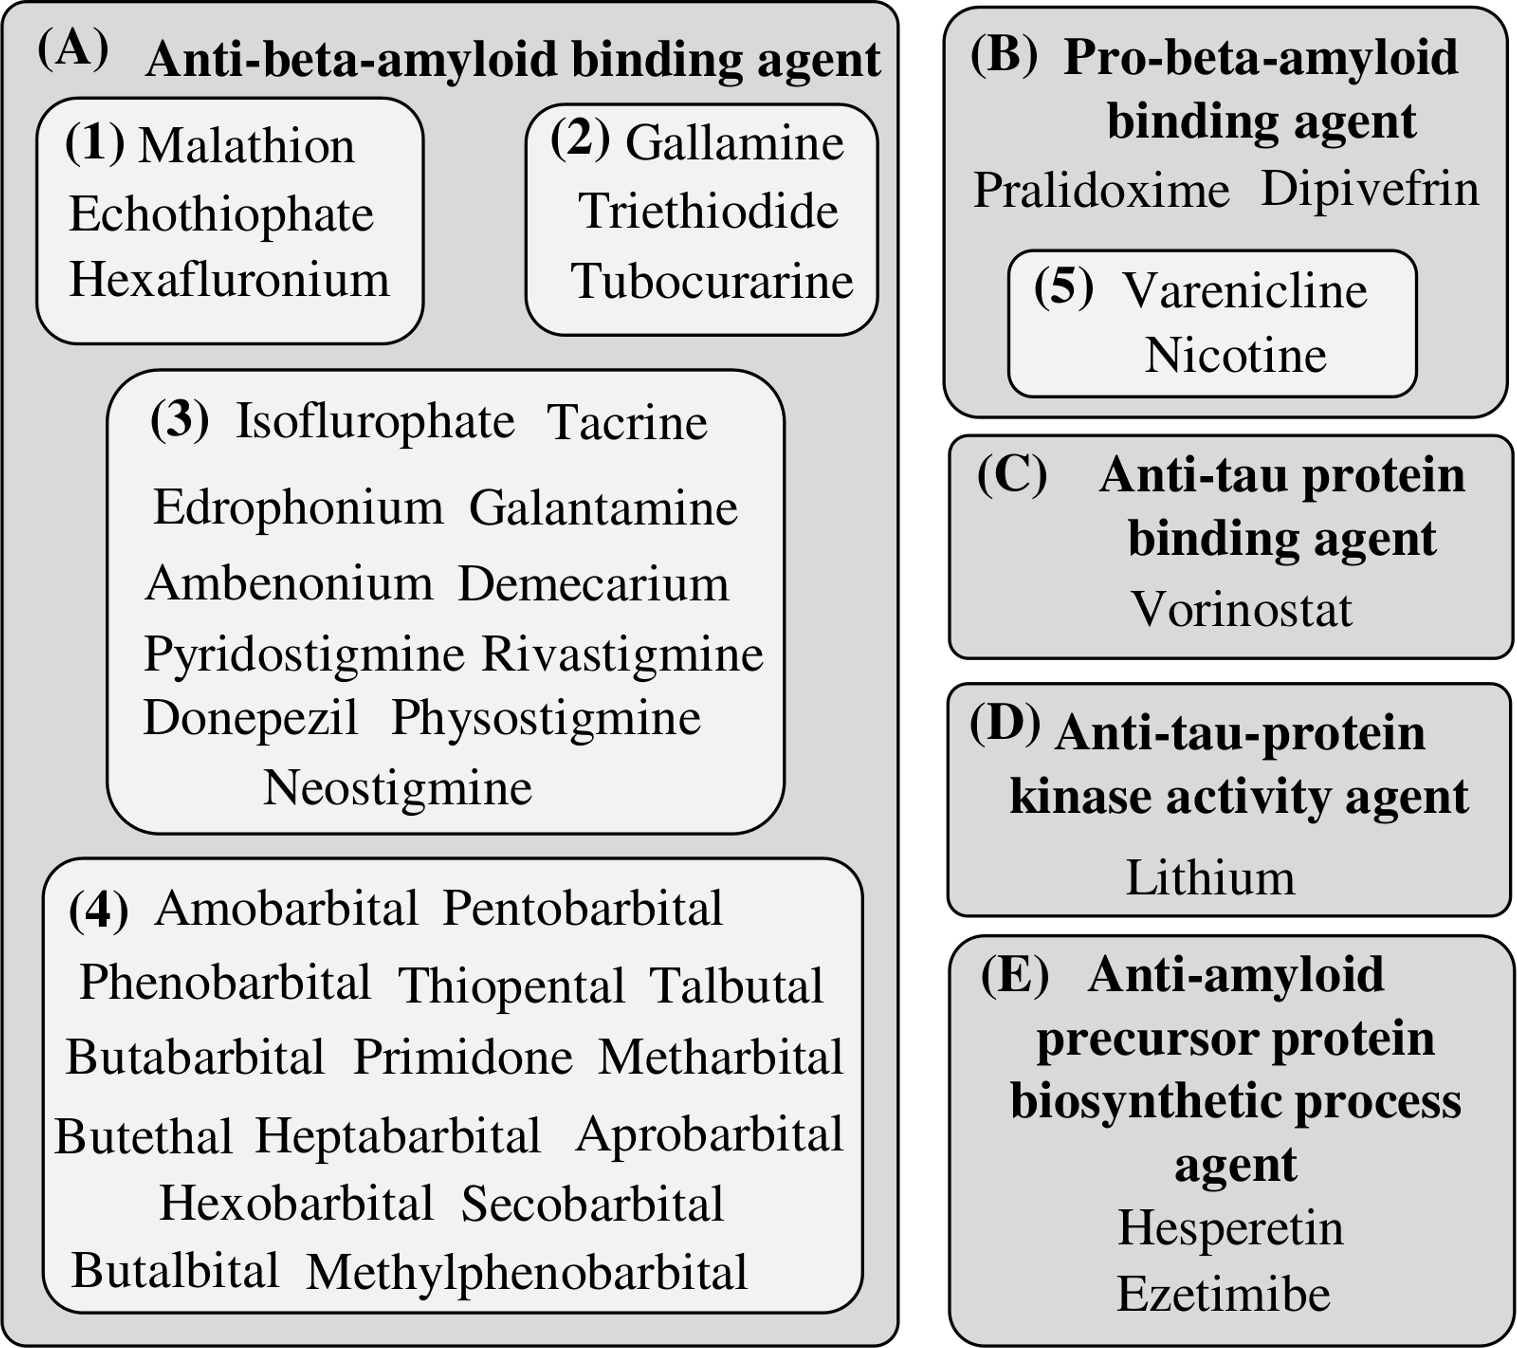
\includegraphics{fig5.png}}
\caption{FTC categories (letters A, F, H, I and J) describing some of the modes and mechanisms of 
action that could impact Alzheimer’s disease. Drugs classified in these FTC categories are listed and further 
manually grouped based on their mode of action similarities (subgroups B, C, D, E and G).}\label{fig:05}
\end{figure}
 
The subgroups B, C and D are inhibitors of the cholinergic system and some of them, such as galantamine (DB00674), are already 
investigated to treat Alzheimer’s disease and other related dementias. This class of agent is in line with the 
cholinergic hypothesis \citep{Francis1999}, stating that Alzheimer’s disease could be caused by dysfunctions in the processing of 
acetylcholine. The subgroup E is exclusively composed of barbiturates (central nervous system depressants). 
The presence of this pharmacological class of compounds as an Alzheimer treatment is more surprising, as very little 
literature reports on it. Further investigations reveal that the neuronal acetylcholine receptor subunit alpha-7, a 
common off-target of barbiturates, binds beta-amyloids with high affinity \citep{Wang2000}. As beta-amyloids are themselves strongly involved 
in the pathology, barbiturates could affect the state of the condition \citep{Wang2000}, similarly to cholinergic inhibitors.
The group F contains four compounds; nicotine and varenicline have been grouped because of similar pharmacology (group G). 
Nicotine has been shown to improve some of the symptoms of Alzheimer’s disease \citep{Jones1992}, it is therefore expected to 
find this molecule in the predictions. Varenicline possess a pharmacology related to that of nicotine, which would explain 
the presence of the drug in this category. The two remaining drugs of group F are respectively pralidoxime and dipivefrin; 
little information is available regarding their potential action against the disease, yet these compounds seem linked to the 
cholinergic hypothesis and could be considered for experimental testing.
The groups H and I contain respectively one molecule each. These compounds have been classified as agents perturbing some of 
the physiological function of the Tau protein, key actor in Alzheimer's disease \citep{Grundke-Iqbal1986}. Vorinostat (group H) is currently 
indicated for the treatment of cutaneous manifestations in patients with T-cell lymphoma, yet a study has 
shown in vivo (mouse model) the potential of the drug and other histone deacetylase inhibitors in regards to memory 
deficit \citep{Kilgore2010}. The presence of lithium (group I) was 
unexpected and suspected of being a false positive at first glance. However a recent study demonstrated a long-term 
protective effect for the ion in regards to Alzheimer’s disease \citep{Young2011}. The last group (J) contains 
ezetimibe and hesperetin. These two compounds are primarily used as cholesterol lowering agents (statins). As cholesterol 
metabolism in the brain appears to be related to dementia, statins are believed to prevent or improve the symptoms of the 
patients. Although early studies \citep{Wolozin2004} have failed to clearly show a beneficial effect, the investigation is still open.
From the examples briefly presented above, reported and confirmed by the literature, the FTC appears to be suitable to 
identify real repurposing hypotheses tailored to a disease. The MoAs help to retrieve the compounds which might impact 
the treatment of a given set of symptoms.

\section{Discussion}

The FTC is a novel classification for approved drugs, which can be used as a starting point to 
generate drug repurposing hypotheses. We have guided the reader through the various ways the resource 
can be explored. No experimental validations have been presented in this manuscript, yet references to 
supporting literature was provided in order to legitimate the claims. The main goal of this document is to 
introduce the resource to the community; deeper analyses are being performed over the classification at the time of writing.

\subsection{Biological assumptions}
An asset of the FTC is its ability to handle efficiently categorical data: Classes and relationships 
are accurately defined, in order to classify compounds based on the semantics of their relations. The properties 
linking drugs to their respective protein targets (positive and negative perturbations) are however simplistic. At the 
time being, no consideration is given regarding the binding strength between the drug and the proteins, yet it is a key 
factor to derive potent and specific activities in the human body. This is also the case for other types of numerical data, 
such as the dosage; the FTC can predict a role for a drug, yet it cannot provide any information about the concentration or 
the administration route necessary to obtain the potential effects. The current relations between targets and their involvement 
in biological processes are also not a fully accurate representation of the biological phenomenon. In a cell, specific domains 
of the protein could mediate different functions. Only one of such activity types can sometimes be inhibited 
by a drug (cite felix paper), yet we are assuming in the FTC that as long as a drug affects a protein, 
it can therefore alter all its known functions.
These limitations come from the semantics behind the axioms structuring the classification, themselves based on the 
information available from the databases (e.g. GOA, DrugBank, etc...). Despite entailing not entirely accurately the 
biochemical reality, the axioms help to generate a larger number of hypotheses, the primary goal of the FTC. The dosage 
issue is partially addressed by the regulator pattern (see section in Availability and Implementation): It should be 
easier to experimentally adjust the concentration of the compounds classified as pro or anti biological process agents 
in order to modulate a physiological effect.
The predictions generated by the FTC depend on the resolution of the curated information released by 
the original data providers. Erroneous or missing information will lead to misclassification by the reasoner. 
Some expected outcomes are also missing from the predictions; sildenafil for instance was expected to be classified 
as pro-penile erection agent (FTC\_A0043084), yet the lack of appropriate GO annotation prevents it. After discussion 
with the GOA curation team, a manual annotation can only be asserted based on published experimental results. No document 
was found to support the involvement of the cGMP-specific 3',5'-cyclic phosphodiesterase (O76074 - sildenafil’s main target) 
in the negative regulation of penile erection (GO:0060407), therefore no annotation can be made. Further work could be done 
in this direction, by trying to automatically infer more annotations or by using the electronically generated ones, in order 
to generate broader yet potentially less plausible repurposing hypotheses.

\subsection{Interpreting the evaluation}
The high recall value (88\%) supports the idea behind the automated build of the FTC: The data from different 
repositories funded and curated in parallel, can be integrated to automatically create a new resource. This new resource (FTC) 
contains most of the known information present in an external gold standard (ATC) and relies on description logics to 
leverage the native information. Here we have assessed the content of the FTC against the ATC, knowing that these two 
taxonomies have diverging goals. During the evaluation, equivalences have been manually asserted between classes, 
which are assumed to have fairly similar meaning and containing similar sets of compounds. These manual assertions 
are however a weakness, as they are themselves not evaluated (free parameter). The presence or absence of a link was 
determined only by one curator and any mistake can influence consequently the recall and precision values. In this regards, 
the evaluation should be considered more as a safety control rather than a formal assessment of a predictive method.
The false positives derived from the evaluation can also be considered as drug repurposing hypotheses: These drugs 
can indeed be interpreted as suitable for the ATC category, yet not indexed as such. However, these predictions 
should be interpreted with caution, as it is currently impossible to distinguish a false positive from a 
reprofiling opportunity. These considerations do not interfere with the repurposing predictions generated 
based on semantic similarities or discrete categories as presented in the Exploration section. Finally, 
note that the ATC/FTC equivalences are open and editable online, any modification will be automatically 
incorporated in the next release of the resource. It is also possible to evaluate the FTC against a different 
taxonomy, like the Medical Subject Headings for example, which can be subject to future work.

\section{Conclusion}
This manuscript introduces the FTC, a free, open and extensible resource, which can assist drug repurposing 
initiatives or enhance computational studies making use of the concept of mode of action. The construction of 
the classification relies on description logics as a means to define the mode and mechanism of action of approved 
drugs. We shown the validity of the approach by comparing the content of the FTC to another well implemented taxonomy, 
the ATC. We further illustrate the tight relationship between the MoA and the indication of a drug and shown how the 
resource can serve as a starting point to formulate hypotheses for Alzheimer's disease. The work leverages the 
semantics of distinct databases, working in parallel on different thematics. The platform will be further used 
to generate predictions in a systematic fashion, which can then be experimentally tested in the laboratory for validation.

\section{Availability and Implementation}
The code behind the creation of the resource is entirely open and available 
at {{https://github.com/loopasam/ftc}}. The web application built on the top of the FTC can be 
find at {{https://www.ebi.ac.uk/chembl/ftc}} and the documentation can be accessed at {{https://github.com/loopasam/ftc/wiki}}. The full
description of the methodology used to generate the classification is available as supplementary material on Bioinformatics website.

\section*{Acknowledgement}
Text Text Text Text Text Text  Text Text.  \citealp{Boffelli03} might want to know about  text text text text

\paragraph{Funding\textcolon} Text Text Text Text Text Text  Text Text.

\bibliographystyle{natbib}
\bibliographystyle{achemnat}
\bibliographystyle{plainnat}
\bibliographystyle{abbrv}
\bibliographystyle{bioinformatics}

\bibliographystyle{plain}

\bibliography{document}


%\begin{thebibliography}{}
%\bibitem[Bardet, 1920]{Bar20}
%Bardet, G. (1920) Sur un syndrome d'obesite infantile avec
%polydactylie et retinite pigmentaire (contribution a l'etude des
%\end{thebibliography}
\end{document}
